%! TEX root = thesis.tex
% vim: ft=tex et sts=2 sw=2

\chapter{Semiclassical physics}
\label{chap04}

\chapterprecishere{%
In this chapter we present a quick rundown of the semiclassical approximation as applied to multicomponent waves.
Using a variational approach, we will derive the ray equations and describe the modifications necessary to extract the bound-state spectrum of a multicomponent wave operator through quantization.
The general theory prescribed in this chapter will form a basis for our study of elastic waves in the next chapter.
\\
}

The study of propagating waves is important to many disciplines across all branches of science and engineering.
A widely employed asymptotic method to solve wave problems is the WKB/semiclassical approximation, which is sometimes also referred to as the eikonal approximation, geometrical optics, etc.
Although the WKB approximation is discussed in almost all books on quantum mechanics, there are several subtle issues, especially when multicomponent waves are involved, that need to be addressed.
Our primary goal in this chapter, therefore, is to review some existing results on the semiclassical approximation as applied to multicomponent wave fields.
In particular, we will derive expressions for two extra phases that appear in the Bohr--Sommerfeld quantization rule for such wave fields.
To keep the exposition simple, we will restrict ourselves to wave equations in one variable.
For more detailed descriptions, we refer to the book by \citet{tracy2014} and references therein.

\section{Introduction}
\label{sec:varintro}

We begin by considering a general wave equation of the form
%
\begin{equation}
  \partial_{t}^{2}\Psi(x,t) + \widehat{\mathsf{H}}\Psi(x,t) = 0,
  \label{eq:full_wave_eq}
\end{equation}
%
where $\Psi(x,t)$ is an $N$-component wave field described by a one-dimensional coordinate $x$ and time $t$.
As as example, in elastodynamics, $\Psi$ is usually composed of displacements from the neutral, undeformed state of some elastic structure, e.g., a rod or a shell.
Also, $\widehat{\mathsf{H}}$ is taken to be a Hermitian operator in the form of an $N\times N$ matrix, composed solely of spatial derivatives (i.e., powers of $\partial_{x}$) with time-independent coefficients.
Assuming that the waves are time harmonic with frequency $\omega$, i.e., $\Psi(x, t) = \psi(x)e^{\pm i\omega t}$, where $\psi(x)$ is the time-independent part of the wave field, Eq.~\eqref{eq:full_wave_eq} can be recast as
%
\begin{equation}
  \widehat{\mathsf{D}}\psi = 0,\quad \text{with}\quad \widehat{\mathsf{D}} = \widehat{\mathsf{H}} - \omega^{2}\mathsf{I}_{N},
  \label{eq:ev_problem}
\end{equation}
%
where $\mathsf{I}_{N}$ is the $N\times N$ identity matrix.

If the coefficients of the spatial derivatives that appear in $\widehat{\mathsf{D}}$ are constants, then the eigenmodes $\psi$ are plain waves.
In what follows we assume that these coefficients are slowly varying, with the variation controlled by a single positive parameter $\epsilon \ll 1$, called the \emph{eikonal parameter}.
It is useful to treat $\epsilon$ as an ordering parameter so that we can look for solutions at various orders of $\epsilon$.
To this end, we rescale $x \to \epsilon^{-1}x$ so that a derivative $\partial_{x}$ becomes $\epsilon \partial x$.
With analogy to quantum mechanics, this allows us to recast the derivatives in $\widehat{\mathsf{D}}$ in terms of the wave number/momentum operator $\hat{k} = -i\epsilon \partial_{x}$, with $\epsilon$ playing the role of Planck's constant.
Since we shall be considering $\widehat{\mathsf{D}}$ in the coordinate representation, the position operator $\hat{x} = x$.

\subsection{Wave action}

Central to the variational approach we will use in this chapter is the realization that
a wave equation like Eq.~\eqref{eq:ev_problem} can be derived from a wave action of the form
%
\begin{equation}
  \begin{aligned}
    \mathscr{U}\left[\psi^{*}, \psi\right] &= \tfrac{1}{2}\bra{\psi}\widehat{\mathsf{D}}\ket{\psi}
  = \tfrac{1}{2}\int \dd{x}\,\dd{x'}\, \braket{\psi|x}\bra{x}\widehat{\mathsf{D}}\ket{x'}\braket{x'|\psi}\\
                                           &= \tfrac{1}{2}\int \dd{x}\dd{x'}\, \psi^{*}_{\mu}(x)\,\widehat{\mathsf{D}}_{\mu\nu}(x, x')\,\psi_{\nu}(x').
  \label{eq:wave_action}
  \end{aligned}
\end{equation}
%
Above we have inserted the resolution of identity $\int \dd{x}\,\ket{x}\bra{x} = 1$ in appropriate places to express $\mathscr{U}$ in terms of $\psi$ and its conjugate $\psi^{*}$.
Also, in the last step, we have made the matrix product between the matrix operator $\widehat{\mathsf{D}}$ and the wave vector $\psi$ explicit, with $\braket{x|\widehat{\mathsf{D}}_{\mu\nu}|x'} = \widehat{\mathsf{D}}_{\mu\nu}(x, x')$ being the matrix element of $\widehat{\mathsf{D}}_{\mu\nu}$ in the position basis.
Varying $\mathscr{U}[\psi^{*}, \psi]$ with respect to $\psi^{*}$ gives the eigenvalue problem, Eq.~\eqref{eq:ev_problem}.
For later use, we also note that $\mathscr{U}$ can also be written as
%
\begin{equation}
  \begin{aligned}
    \mathscr{U}\left[\psi^{*}, \psi\right] &= \tfrac{1}{2}\int \dd{x}' \braket{\psi_{\mu}|x'}\bra{x'}\widehat{\mathsf{D}}_{\mu\nu}\ket{\psi_{\nu}}
= \tfrac{1}{2}\int \dd{x}' \bra{x'}\widehat{\mathsf{D}}_{\mu\nu}\ket{\psi_{\nu}} \braket{\psi_{\mu}|x'}\\
&= \tfrac{1}{2}\int \dd{x}' \bra{x'}\widehat{\mathsf{D}}_{\mu\nu}\widehat{\mathsf{W}}_{\nu\mu}\ket{x'} = \tfrac{1}{2}\tr\left(\widehat{\mathsf{D}}_{\mu\nu}\widehat{\mathsf{W}}_{\nu\mu}\right),
  \label{eq:wave_action_trace_form}
  \end{aligned}
\end{equation}
%
where the matrix operator
%
\begin{equation}
  \widehat{\mathsf{W}}_{\nu\mu} = \ket{\psi_{\nu}}\bra{\psi_{\mu}},
\end{equation}
%
is the density operator.

In order to solve Eq.~\eqref{eq:ev_problem} at various orders of $\epsilon$, it is convenient to make use of Weyl calculus, which allows one to map differential operators that are functions of $\hat{x}$ and $\hat{k}$ to ordinary functions, called Weyl symbols, defined on an $x$-$k$ phase space, and vice versa~\cite{chaichian2001,cohen2012}.
For the purposes of this chapter, the following simple rules suffice to convert operators to symbols:
%
\begin{equation}
  f(x) \to f(x),\enspace
  g(\hat{k}) \to g(k),\enspace\text{and}\enspace
  f(x)g(\hat{k}) \to f(x)g(k) + \frac{i\epsilon}{2}f'(x)g'(k) + \mathcal{O}(\epsilon^{2}).
  \label{eq:weylrules}
\end{equation}
%
Above, $f$ and $g$ are functions of $x$ and $\hat{k}$, with the primes denoting derivatives.
Converting each entry of the matrix operator $\widehat{\mathsf{D}}$ into a Weyl symbol, we get the $N\times N$ dispersion matrix $\mathsf{D}$, which we express in various orders of $\epsilon$ as $\mathsf{D} = \mathsf{D}^{(0)} + \epsilon\mathsf{D}^{(1)} + \mathcal{O}(\epsilon^{2})$.

The Wigner tensor $\mathsf{W}_{\nu\mu}$ is defined as the symbol of the density operator $\widehat{\mathsf{W}} = \ket{\psi}\bra{\psi}$ with kernel $\widehat{\mathsf{W}}_{\nu\mu}(x',x) = \psi_{\nu}(x')\psi_{\mu}^{*}(x)$, and is given by
%
\begin{equation}
  \mathsf{W}_{\nu\mu}(x, k) = \int \dd{s}\, e^{-iks/\epsilon}\, \psi_{\nu}\left(x + \tfrac{1}{2}s\right)\psi^{*}_{\mu}\left(x - \tfrac{1}{2}s\right).
\end{equation}
%
By inverting the above expression, and setting $x + \tfrac{1}{2}s \to x'$ and $x- \tfrac{1}{2}s \to x$, we can write the kernel of the density operator in terms of its Weyl symbol as
%
%\begin{equation}
%  \psi_{k}\left(x + \tfrac{1}{2}s\right) \psi^{*}_{j}\left(x - \tfrac{1}{2}s\right) = \frac{1}{2\pi \epsilon} \int \dd{k}\, e^{iks/\epsilon}\,\mathsf{W}_{\nu\mu}(x, k).
%\end{equation}
%%
%so that
%
\begin{equation}
  \psi_{\nu}(x') \psi^{*}_{\mu}(x) = \frac{1}{2\pi \epsilon} \int \dd{k}\, e^{ik(x' -x)/\epsilon}\,\mathsf{W}_{\nu\mu}\left[\tfrac{1}{2}(x' + x), k\right].
  \label{eq:density_operator}
\end{equation}
%
In a similar fashion, we find
%
\begin{equation}
  \widehat{\mathsf{D}}_{\mu\nu}(x, x') = \frac{1}{2\pi\epsilon} \int \dd{l}\, e^{il(x -x')/\epsilon}\,\mathsf{D}_{\mu\nu}\left[\tfrac{1}{2}(x + x'), l\right].
  \label{eq:Dhat_integral}
\end{equation}
%
Putting Eq.~\eqref{eq:Dhat_integral} and \eqref{eq:density_operator} in Eq.~\eqref{eq:wave_action}, we arrive at
%
\begin{equation}
  \mathscr{U} = \frac{1}{2(2\pi\epsilon)^{2}}\int \dd{x}\,\dd{x'}\,\dd{k}\,\dd{l}\, e^{i(l-k)(x -x')/\epsilon}\,\mathsf{D}_{\mu\nu}\left[\tfrac{1}{2}(x + x'), l\right]\, \mathsf{W}_{\nu\mu}\left[\tfrac{1}{2}(x' + x), k\right].
\end{equation}
%
Performing the change of variables $x \to \tfrac{1}{2}(x + x')$ and $x' \to x - x'$, which carries a Jacobian factor of unity, we arrive at
%
\begin{equation}
  \begin{aligned}
    \mathscr{U} &= \frac{1}{2(2\pi\epsilon)^{2}}\int \dd{x}\,\dd{x'}\,\dd{k}\,\dd{l}\, e^{i(l-k)x'/\epsilon}\,\mathsf{D}_{\mu\nu}(x, l)\,\mathsf{W}_{\nu\mu}(x, k)\\
                &= \frac{1}{4\pi\epsilon}\int \dd{x}\,\dd{k}\,\mathsf{D}_{\mu\nu}(x, k)\,\mathsf{W}_{\nu\mu}(x,k)\\
  \end{aligned}
  \label{eq:wave_action_symbol_form}
\end{equation}

So far there has been no approximations involved and the wave action in Eq.~\eqref{eq:wave_action_symbol_form} is exact to all orders of the eikonal parameter.
That said, the curious reader may wonder there is an inconsistency here, in light of Eq.~\eqref{eq:wave_action_trace_form}, where we have expressed $\mathscr{U}$ as the trace of the (scalar) operator $\widehat{O} = \widehat{\mathsf{D}}_{\mu\nu}\widehat{\mathsf{W}}_{\nu\mu}$.
In terms of its symbol, the trace of an operator $\widehat{O}$ is
%
\begin{equation}
  \tr\widehat{O} = \frac{1}{2\pi\epsilon} \int \dd{x}\,\dd{k}\, O(x, k),
\end{equation}
%
so that $\mathscr{U}$ must be
%
\begin{equation}
  \mathscr{U} = \tr{\widehat{O}} = \frac{1}{4\pi\epsilon}\int \dd{x}\,\dd{k}\, \mathsf{D}_{\mu\nu}(x,k)e^{i\widehat{\mathcal{L}}}\mathsf{W}_{\nu\mu}(x, k),
\end{equation}
%
where we have used the Moyal formula to write the symbol $O$ in terms of the symbols of $\mathsf{D}_{\mu\nu}$ and $\mathsf{W}_{\nu\mu}$.
The issue here is a bit subtle---the resolution is that each correction term in the Moyal series can be expressed as divergence of a vector field in the $(x, k)$ phase space~\cite[Problem 3.16]{tracy2014}.
Hence, using the divergence theorem, the integrals over the correction terms vanish for all well-behaved wave fields.
Thus, only the first term in the Moyal series remains, and we get Eq.~\eqref{eq:wave_action_symbol_form} again.

Returning to our main problem, i.e., to employ the semiclassical approximation to solve Eq.~\eqref{eq:ev_problem}, we will proceed as follows: (i) insert the eikonal ansatz into the wave action; (ii) expand the action to the lowest order in the eikonal parameter and form the \emph{reduced action} $\mathscr{U}_{\text{R}}$; (iii) extract the semiclassical equations of motions by varying the reduced action.

\subsubsection*{Reduced wave action}
\label{page:redaction}

As we have assumed that the coefficients of the differential operators in $\widehat{\mathsf{D}}$ are slowly varying, it makes sense to look for an almost plain-wave-like solution of the form
$\psi(x) = A(x)e^{iS(x)/\epsilon}$, where the amplitude $A(x)$ is an $N$-component spinor with complex components, and $S(x)/\epsilon$ is a rapidly varying phase, playing the role of an action.
This is the \emph{eikonal} ansatz, and the parameter $\epsilon$ that controls the slowness of the variation is the eikonal parameter.
To employ the eikonal ansatz, we set $\psi_{\mu} = A_{\mu}e^{iS(x)/\epsilon}$ in Eq.~\eqref{eq:wave_action_symbol_form} to obtain%
%
\begin{equation}
    \mathsf{W}_{\nu\mu}(x, k) = \int \dd{r}\,e^{-ikr/\epsilon} A_{\nu}\left(x + \tfrac{1}{2} r\right)A_{\mu}^{*}\left(x - \tfrac{1}{2} r\right)\exp\left\{\frac{i}{\epsilon}\left[S\left(x + \tfrac{1}{2} r\right) - S\left(x - \tfrac{1}{2} r\right)\right]\right\}.
\end{equation}
%
Next, we set $r \to \epsilon r$ and expand the amplitude $A_{\nu}(x + \tfrac{1}{2}\epsilon r) = A_{\nu}(x) + \tfrac{1}{2}(\partial_{x}A_{\nu})\epsilon r + \mathcal{O}(\epsilon^{2})$ and the phase $S(x + \tfrac{1}{2}\epsilon r) = S(x) + \tfrac{1}{2}[\partial_{x}S(x)]\epsilon r + \mathcal{O}(\epsilon^{2})$ to obtain
%
\begin{equation}
  \begin{aligned}
    \mathsf{W}_{\nu\mu}(x, k) &= \epsilon\int \dd{r}\,e^{-ikr} A_{\nu}(x)A_{\mu}^{*}(x)\exp\left\{ir\left[\partial_{x}S(x) - k\right]\right\} + \mathcal{O}(\epsilon^{2}) \\
                        &= 2\pi\epsilon A_{\nu}(x)A^{*}_{\mu}(x)\delta\left[k - \partial_{x}S(x)\right] + \mathcal{O}(\epsilon^{2}).
  \end{aligned}
\end{equation}
%
We assume that the dispersion matrix is ordered in the eikonal parameter $\epsilon$ so that we can write
$\mathsf{D} = \mathsf{D}^{(0)} + \epsilon \mathsf{D}^{(1)} + \mathcal{O}(\epsilon^{2})$.
Hence, after putting the ``reduced'' Wigner tensor in Eq.~\eqref{eq:wave_action_symbol_form}, we find the action to the lowest order as
%
\begin{equation}
  \mathscr{U} = \tfrac{1}{2}\int \dd{x}\, \mathsf{D}^{(0)}_{\mu\nu}\left[x, k=\partial_{x}S(x)\right]A_{\nu}(x)A^{*}_{\mu}(x) + \mathcal{O}(\epsilon^{2}).
  \label{eq:wave_action_reduced_1}
\end{equation}
%
Next, we perform a spectral decomposition of the lowest-order dispersion matrix $\mathsf{D}^{(0)}_{\mu\nu}(x, k)$ and write it in terms of its eigenvectors $\tau_{a}$ and eigenvalues $\lambda_{a}$ as%
\footnote{In Eq.~\eqref{eq:Dmat_polarization}, the subscripts $\mu$ and $\nu$ indicate the components of $\tau_{a}$.
Also, we have made the summation over the polarization index $a$ explicit---a convention that we will use throughout this dissertation.}
%
\begin{equation}
  \mathsf{D}^{(0)}_{\mu\nu}(x, k) = \sum_{a} \lambda_{a}(x, k) \tau_{a, \mu}(x, k) \tau_{a, \nu}^{*}(x, k).
  \label{eq:Dmat_polarization}
\end{equation}
%
An eigenvector $\tau_{a}$ describes a specific wave type or ``polarization'' represented by the wave equation, Eq.~\eqref{eq:ev_problem}.
And by polarization, we mean a linear subspace of the total wave field that is usually of a distinct physical nature, e.g., flexural waves on a rod.

We put Eq.~\eqref{eq:Dmat_polarization} into Eq.~\eqref{eq:wave_action_reduced_1}, and define $B_{a} = \tau_{a, \nu}^{*}A_{\nu} = \braket{\tau_{a}|A}$, which is the projection of the amplitude $A_{\nu}$ along the direction of the polarization vector $\tau_{a}$.
Although both $A_{\nu}$ and $\tau_{a}$ are general complex vectors, we can take the scalar projection $B_{a}$ to be positive by absorbing the complex phase of $A_{\nu}$ into $\tau_{a}$.
This results in a reduced action of the form
%
\begin{equation}
  \mathscr{U}_{\text{R}}\left[B_{a}, S\right] = \tfrac{1}{2} \sum_{a} \int \dd{x}\, \lambda_{a}(x,k) B_{a}^{2}(x, k),
  \quad\text{with}\quad
  k = \partial_{x}S(x).
  \label{eq:reduced_action}
\end{equation}

\subsection{Phase-space representation of waves}

Variation of the reduced action, Eq.~\eqref{eq:reduced_action}, with respect to the amplitude $B_{a}$ yields
%
\begin{equation}
  \lambda_{a}[x, k(x)]\,B_{a}[x, k(x)] = 0
  \quad\text{for all $a$}.
\end{equation}
%
Assume that the amplitudes $B_{a}$ is nonzero only for one polarization, say, $a = I$, which means that the corresponding eigenvalue must vanish, yielding
%
\begin{equation}
  \lambda_{I}\left[x, k(x)\right] = \lambda_{I}\left[x, \partial_{x}S(x)\right] = 0.
  \label{eq:eikonal}
\end{equation}
%
The above equation, which is known as the eikonal equation, is nothing but the Hamilton--Jacobi equation with $S(x)$ playing the role of the classical action.
 This leads us to the phase-space representation of waves as rays that satisfy the Hamilton's equations
%
\begin{equation}
  \frac{\dd{x}}{\dd{\sigma}} = \partial_{k}\lambda_{I}(x, k) = \left\{x, \lambda_{I}\right\}
  \quad\text{and}\quad
  \frac{\dd{k}}{\dd{\sigma}} = -\partial_{x}\lambda_{I}(x, k) = \left\{k, \lambda_{I}\right\},
\end{equation}
%
where $\sigma$ is some parameter that parameterizes the rays $[x(\sigma), k(\sigma)]$ in the phase space, and $\left\{\cdot, \cdot\right\}$ is the $x$-$k$ Poisson bracket.
Since the waves we consider propagate in a one-dimensional space, these rays are identical to the level curve defined by $\lambda_{I}(x, k) = 0$.

In higher dimensions, solving the Hamilton-Jacobi equation can be nontrivial.
However, in one dimension, it is always theoretically possible to solve for $k(x)$ from $\lambda_{I}(x, k) = 0$.
% TODO: Tori... quantization, more stuff about Hamilton-Jacobi equations.
Variation of the action, Eq.~\eqref{eq:reduced_action}, with respect to the phase $S(x)$ yields the amplitude transport equation%
\footnote{Here we have ignored the term $\partial_{k}{B_{I}^{2}(x,k)}\lambda_{I}$, which trivially vanishes as $\lambda_{I}(x, k) = 0$ on an orbit.
Also, since $k$ is a function of $x$ on an orbit, we can simply write the projected amplitude as $B(x)$ instead of $B(x,k)$.
Note also that after evaluating the partial derivative of $\lambda_{I}$ with respect to $k$, we need to set $k \to k(x)$ for the full derivative with respect to $x$ to make sense.}
%
\begin{equation}
  \frac{\dd}{\dd{x}}\left[B^{2}_{I}(x)\partial_{k}\lambda^{(0)}_{I}(x, k)\right] = 0
\end{equation}
%
so that
$B^{2}(x,k)\partial_{k}\lambda^{(0)}_{I}(x, k) = C$ (constant) and
%
\begin{equation}
  B_{I}(x) = \frac{C}{\sqrt{\partial_{k}\lambda_{I}(x, k)}}.
\end{equation}
%
Clearly, the amplitude projection $B_{I}$ becomes singular at points on the phase space where $\dot{x} = \partial_{k}\lambda_{I}(x, k) = 0$, i.e., when the local tangent along a ray points along the $k$ axis.
Such points are called caustics, and they arise because of ill-defined projections from the ray, which lives in the $x$-$k$ phase space, to the coordinate space, i.e., $x$ space.
The issue can be sidestepped using the Keller--Maslov method~\cite{keller1958,maslov1981} where one Fourier transforms the wave field and uses the eikonal ansatz in the momentum space.
Although we shall later rely on some results of this procedure, we will not discuss its technical details here.
Interested readers are encouraged to look at the book by \citet[Chapter 6]{tracy2014} (and references therein) for more information.

In writing down the eikonal equation, Eq.~\eqref{eq:eikonal}, we have assumed that the amplitude projection $B_{a} \neq 0$ only for $a = I$.
Now, as $\mathsf{D}^{(0)}$ is a Hermitian matrix, its eigenvectors $\tau_{a}$ are mutually orthogonal, and the wave amplitude $A_{\mu} = \sum_{a} B_{a} \tau_{a,\mu} = B_{I}\tau_{I,\mu}$.
This would clearly be wrong if the matrix $\mathsf{D}^{(0)}$ is degenerate.
For this reason, usual semiclassical solutions also break down near points in the phase-space where more than one eigenvalue of $\mathsf{D}^{(0)}$ simultaneously vanish, leading to a exchange of energy and mode conversion between waves of different polarizations~\cite{tracy2014}.
As the wave problems we study in this dissertation do not suffer from mode-conversion issues (at least in the parameter ranges we are interested in), we forgo a more detailed discussion on these issues here.

Assuming that we are far away from caustics and ignoring mode-conversion effects, we can write the final eikonal solution as
%
\begin{equation}
  \psi_{\mu}(x) \sim B_{I}[x, k(x)]\,\tau_{I,\mu}[x, k(x)]e^{iS(x)/\epsilon}.
  \label{eq:psi_wkb_wrong}
\end{equation}
%
At this juncture, we must discuss a subtle problem.
The polarization vector $\tau_{I}$ is only defined up to an overall phase.
Thus, instead of the above equation, it is more appropriate to write
%
\begin{equation}
  \psi_{\mu}(x) \sim B_{I}[x, k(x)]\,\tau_{I,\mu}e^{i\gamma[x, k(x)]}e^{iS(x)/\epsilon},
\end{equation}
%
where $\gamma[x, k(x)]$ stands for an adiabatic phase that we have not determined so far.
As $\tau_{I}$ is obtained from $\mathsf{D}^{(0)}$, whose entries are slowly varying functions of $(x, k)$, it makes sense to consider the phase $\gamma[x, k(x)]$ to be slowly varying as well.
For this reason, $\gamma$ cannot be absorbed into the eikonal phase $S(x)/\epsilon$, which is rapidly varying.

The phase $\gamma$ becomes important when quantizing orbits---a step that boils down to the single valuedness of $\psi_{\mu}$ as we move around a closed orbit, i.e., the sum of $\gamma$ and $S/\epsilon$ must be a half-integral multiple of $2\pi$ (see Section~\ref{sec:bound}).
Unfortunately, our lowest-order analysis is insufficient to determine this phase.
We cannot also find an evolution equation for this phase from the reduced action, Eq.~\eqref{eq:reduced_action}, as it is independent of $\gamma$.
It can also be easily checked that the phase $\gamma$ cannot be introduced in the action by rephasing $\tau$ by the phase factor $e^{i\gamma(x,k)}$, as the action remains invariant.
The message is clear: to find $\gamma$, we need to include higher-order corrections in the wave action.
To this end, rather than repeat the original, but cumbersome derivations scattered across Refs.~\cite{bernstein1975,berk1980,yabana1986,kaufman1987}, it is more sagacious to switch gears and follow a different approach due to Littlejohn and coworkers~\cite{littlejohn1991,littlejohn1991a} for (approximately) diagonalizing multicomponent differential operators.

%Employing the eikonal ansatz, at $\mathcal{O}(\epsilon^{0})$, we find the matrix equation $\mathsf{D}^{(0)}A = 0$.
%To satisfy this equation, at least one of the $N$ eigenvalues of $\mathsf{D}^{(0)}$, say $\lambda(x, k;\, \omega)$, must vanish so that $\det \mathsf{D}^{(0)}(x, k; \omega) = 0$.
%A vanishing eigenvalue $\lambda$ and the associated normalized eigenvector $\tau$ describes different wave types or ``polarizations'' represented by Eq.~\eqref{eq:ev_problem}.
%By a polarization we mean a linear subspace of the total wave field that is usually of a distinct physical nature, e.g., flexural waves on a curved rod.
%Semiclassical approximation breaks down near points where more than one eigenvalues of $\mathsf{D}^{(0)}$ simultaneously vanish, precipitating an exchange of energy and mode conversion between waves of different polarizations~\cite{tracy2014}.

%In the absence of mode conversion, the vanishing eigenvalues of $\mathsf{D}^{(0)}$ also serve as the \emph{ray Hamiltonian} of waves of a specific polarization.
% This leads us to the phase-space representation of waves as rays that satisfy the Hamilton's equations
%%
%\begin{equation}
%  \dot{x} = \partial_{k} \lambda(x, k;\, \omega) = \left\{x, \lambda\right\}
%  \quad\text{and}\quad
%  \dot{k} = -\partial_{x} \lambda(x, k;\, \omega) = \left\{k, \lambda\right\},
%\end{equation}
%%
%where the overdot denotes derivatives with respect to a parameter that parameterizes the rays and $\left\{\cdot, \cdot\right\}$ is the $x$-$k$ Poisson bracket.
%Since the waves we consider propagate in a one-dimensional space, these rays are identical to the level curve defined by $\lambda(x, k; \omega) = 0$.
%%
% \begin{figure}
%   \begin{center}
%     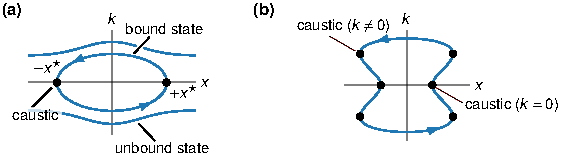
\includegraphics{localization/caustic.pdf}
%   \end{center}
%   \caption{%
%     (a) In phase space, bound states are represented by rays in the form of closed orbits, which is analogous to that of a bound particle oscillating between two classical turning points ($\pm x^{\star}$ in the cartoon).
%     Other trajectories represent unbound states.
%     (b) A bound state represented by a ``peanut''-shaped orbit has six caustics.%
%   }
%   \label{fig:caustic}
% \end{figure}

%%
%\begin{equation}
%\gamma_{\text{G}} = \oint \dd{\sigma}\, \dot{\gamma}_{\text{G}} = i\oint \dd{\sigma}\,\left\langle{\tau_{a}}\middle|\dot{\tau}_{\alpha}\right\rangle =
%  i\oint \dd\xi\cdot\left\langle{\tau_{a}}\middle|\nabla_{\xi}\tau_{\alpha}\right\rangle,
%\end{equation}
%%
%where $\xi = (x, k)$ denotes the ``parameters'' that are being varied.

%%In Appendix~\ref{app:additional_phase} we prove that $\gamma_{\text{G}}$ vanishes if the relative phases between the components of the eigenvector $\tau_{a}$ are constants.
%%The second (non-geometric) phase $\gamma_{\text{NG}}$ need not vanish in such a situation, however.
%Instead of explicitly accounting for the extra phase $\gamma$ in the quantization rule, we could have diagonalized the wave equation at various orders of $\epsilon$~\cite{littlejohn1991,littlejohn1991a,weigert1993,venaille2023}.
%During such a procedure, terms proportional to $\dot{\gamma}_{\text{G}}$ and $\dot{\gamma}_{\text{NG}}$ naturally appear in the ray Hamiltonian $\lambda$ as a first-order correction.
%Despite the elegance of the method, we do not use it in our analysis.
%This is because, as we discuss in Appendix~\ref{app:additional_phase}, for both the problems we consider, the extra phases vanish.


\section{Intermission: diagonalizing multicomponent operators}
\label{sec:diagonalize}

We start again, with a Hermitian linear differential operator $\widehat{\mathsf{D}}$ in the form of an $N\times N$ matrix satisfying a wave equation
%
\begin{equation}
  \widehat{\mathsf{D}}\Psi = 0,
\end{equation}
%
where $\Psi$ is an $N$-component wave field.
%
We want to find a unitary operator $\widehat{\mathsf{U}}$ such that
%
\begin{equation}
  \widehat{\mathsf{U}}^{\dagger}\widehat{\mathsf{D}}\widehat{\mathsf{U}} = \widehat{\Lambda}\label{eq:diagonalization}
\end{equation}
%
is a diagonal operator.
Clearly, this equivalent to demanding that $\widehat{\mathsf{D}}\widehat{\mathsf{U}} = \widehat{\mathsf{U}}\widehat{\Lambda}$.
If we can find such an operator and solve the decoupled set of equations given by $\widehat{\Lambda}\Phi = 0$ somehow,
the solutions to the original equation can then be recovered from $\Phi$ using $\Psi = \widehat{\mathsf{U}}\Phi$.
However, Eq.~\eqref{eq:diagonalization} is an equation involving operator products and standard linear algebra methods do not (directly) help in finding the unitary operator $\widehat{\mathsf{U}}$.
Instead, we start by finding the symbol form of the following two equations:
%
\begin{equation}
  \begin{aligned}
    \widehat{\mathsf{D}}\widehat{\mathsf{U}} &= \widehat{\mathsf{U}}\widehat{\Lambda}\\
    \widehat{\mathsf{U}}^{\dagger}\widehat{\mathsf{U}} &= \hat{\mathsf{I}}_{N}.
  \end{aligned}
  \label{eq:diagonal2}
\end{equation}
%
Here we assume that the operators $\widehat{\mathsf{D}}$, $\widehat{\mathsf{U}}$, and $\widehat{\Lambda}$ have some problem-relevant ordering parameter $\epsilon$ so that we can expand%
\footnote{In their papers, Littlejohn and coworkers~\cite{littlejohn1991,weigert1993} assume that $\widehat{\mathsf{D}}$ is \emph{not} ordered in $\epsilon$, i.e., $\widehat{\mathsf{D}} = \widehat{\mathsf{D}}_{0}$.
  This might seem confusing at first since the parameter $\epsilon$ must appear somewhere in the problem.
  The thing is that very often, $\epsilon$ appears as a factor to a spatial derivative operator, e.g., $\epsilon\partial_{x}$, which once expressed in terms of the momentum operator, does not have additional dependence on $\epsilon$.
  Of course, $\widehat{\mathsf{D}}$ could have further nontrivial dependence on $\epsilon$, which is a more general situation, and the one we want to consider here.
}
the operators (and their symbols) in terms of $\epsilon$ as follows:
%
\begin{equation}
  \begin{aligned}
    \widehat{\mathsf{D}} &= \widehat{\mathsf{D}}^{(0)} + \epsilon\widehat{\mathsf{D}}^{(1)} + \epsilon^{2}\widehat{\mathsf{D}}^{(2)} + \cdots\\
    \widehat{\mathsf{U}} &= \widehat{\mathsf{U}}^{(0)} + \epsilon\widehat{\mathsf{U}}^{(1)} + \epsilon^{2}\widehat{\mathsf{U}}^{(2)} + \cdots\\
    \widehat{\Lambda} &= \widehat{\Lambda}^{(0)} + \epsilon\widehat{\Lambda}^{(1)} + \epsilon^{2}\widehat{\Lambda}^{(2)} + \cdots
  \end{aligned}
  \qquad\text{and}\qquad
  \begin{aligned}
    {\mathsf{D}} &= {\mathsf{D}}^{(0)} + \epsilon{\mathsf{D}}^{(1)} + \epsilon^{2}{\mathsf{D}}^{(2)} + \cdots\\
    {\mathsf{U}} &= {\mathsf{U}}^{(0)} + \epsilon{\mathsf{U}}^{(1)} + \epsilon^{2}{\mathsf{U}}^{(2)} + \cdots\\
    {\Lambda} &= {\Lambda}^{(0)} + \epsilon{\Lambda}^{(1)} + \epsilon^{2}{\Lambda}^{(2)} + \cdots
  \end{aligned}
\end{equation}
%
Because the Weyl transform preserves Hermiticity, $\mathsf{D}$ is a Hermitian matrix to all orders.
Our requirement is that $\Lambda$ remains diagonal at all orders of $\epsilon$.
To proceed, we use the Moyal star product to find the symbol form of Eq.~\eqref{eq:diagonal2} at different orders of $\epsilon$.
At $\mathcal{O}(\epsilon^0)$ we find $\mathsf{D}^{(0)}\mathsf{U}^{(0)} = \mathsf{U}^{(0)}\Lambda^{(0)}$ and $\mathsf{U}^{(0)\dagger}\mathsf{U}^{(0)} = \mathsf{I}_{n}$, with the first equation being equivalent to
%
\begin{equation}
  \mathsf{U}^{(0)\dagger}\mathsf{D}^{(0)}\mathsf{U}^{(0)} = \Lambda^{(0)}.\label{eq:omega0}
\end{equation}
%
Since we demand $\Lambda^{(0)}$ to be diagonal, this is the usual linear algebra problem of diagonalizing the matrix $\mathsf{D}^{(0)}$.
We thus deduce that the columns of the matrix $\mathsf{U}^{(0)}$ are composed of eigenvectors $\tau_{a}$ with eigenvalues $\lambda^{(0)}_{a}$ satisfying $\mathsf{D}^{(0)}\tau_{a} = \lambda^{(0)}_{a}\tau_{a}$, with $a = 1,2,\ldots,N$.
More explicitly,
%
\begin{equation}
  \mathsf{U}^{(0)} =
  \begin{pmatrix}
    \tau_{1} & \tau_{2} & \cdots & \tau_{n}
  \end{pmatrix}.
\end{equation}
%
The matrix $\Lambda^{(0)} = \diag(\lambda_{1}^{(0)}, \lambda_{2}^{(0)}, \ldots, \lambda_{N}^{(0)})$ is composed of the eigenvalues $\lambda_{a}^{(0)}$.

At $\mathcal{O}(\epsilon^{1})$, demanding $\mathsf{D}\mathsf{U} = \mathsf{U}\Lambda$ gives us
%
\begin{equation}
\mathsf{D}^{(1)}\mathsf{U}^{(0)} + \mathsf{D}^{(0)}\mathsf{U}^{(1)} + (i/2)\left\{\mathsf{D}^{(0)}, \mathsf{U}^{(0)}\right\} =
  \mathsf{U}^{(1)}\Lambda^{(0)} + \mathsf{U}^{(0)}\Lambda^{(1)} + (i/2)\left\{\mathsf{U}^{(0)}, \Lambda^{(0)}\right\}.
\end{equation}
%
Multiplying from the left by $\mathsf{U}^{(0)\dagger}$ and making use of $\mathsf{U}^{(0)\dagger}\mathsf{D}^{(0)} = \Lambda^{(0)}\mathsf{U}^{(0)\dagger}$, we get the $\mathcal{O}(\epsilon)$ correction%
\footnote{For further higher-order corrections to $\Lambda$, see Eq.~(19) of Ref.~\cite{weigert1993}.}
%
\begin{equation}
  \Lambda^{(1)} = \left(\mathsf{U}^{(0)\dagger}\mathsf{D}^{(1)}\mathsf{U}^{(0)} +
  (i/2)\mathsf{U}^{(0)\dagger}\left\{\mathsf{D}^{(0)},\mathsf{U}^{(0)}\right\} - (i/2)\mathsf{U}^{(0)\dagger}\left\{\mathsf{U}^{(0)},\Lambda^{(0)}\right\}\right) + \left[\Lambda^{(0)},\mathsf{U}^{(0)\dagger}\mathsf{U}^{(1)}\right].
  \label{eq:Lambda1}
\end{equation}
%
Above $[\cdot,\cdot]$ denotes the matrix commutator.
We can find $\mathsf{U}^{(0)}$ and $\Lambda^{(0)}$ by diagonalizing $\mathsf{D}^{(0)}$.
The matrix $\mathsf{D}^{(1)}$ (if it is nonzero) can be found by expanding the symbol matrix $\mathsf{D}$.
But that will still not let us find $\Lambda^{(1)}$ since we also need $\mathsf{U}^{(1)}$ to evaluate the commutator term $[\Lambda^{(0)},\mathsf{U}^{(0)\dagger}\mathsf{U}^{(1)}]$.
To proceed, we recall that we want $\Lambda$ to be diagonal at all orders, which means that $\Lambda^{(1)}$ must be a diagonal matrix as well.
The $ab$th entry of the commutator term evalutes to
%
\begin{equation}
%  \begin{aligned}
    \left[\Lambda^{(0)},\mathsf{U}^{(0)\dagger}\mathsf{U}^{(1)}\right]_{ab} = %\Lambda_{0,\alpha\gamma}\left(\mathsf{U}^{(0)\dagger}\mathsf{U}^{(1)}\right)_{\gammab} -
  %\left(\mathsf{U}^{(0)\dagger}\mathsf{U}^{(1)}\right)_{a\gamma}\Lambda_{0,\gammab}\\
    %&= \lambda_{0}^{(i)}\delta_{a\gamma}\left(\mathsf{U}^{(0)\dagger}\mathsf{U}^{(1)}\right)_{\gammab}
  %-\left(\mathsf{U}^{(0)\dagger}\mathsf{U}^{(1)}\right)_{a\gamma} \lambda_{0}^{(k)}\delta_{\gammab}\\
    \left[\lambda^{(0)}_{a} - \lambda^{(0)}_{b}\right]\left(\mathsf{U}^{(0)\dagger}\mathsf{U}^{(1)}\right)_{ab},
%  \end{aligned}
    \label{eq:diagonal}
\end{equation}
%
where we have made use of the fact that $\Lambda^{(0)}$ is diagonal so that $\Lambda^{(0)}_{ab} = \lambda^{(0)}_{a}\delta_{ab}$.
And we see that the diagonal entries (with $a=b$) of the commutator vanish.
So the commutator term does not contribute towards the diagonal entries of $\Lambda^{(1)}$ and we can find the $\mathcal{O}(\epsilon^{1})$ correction $\lambda^{(1)}_{a}$ to the eigenvalues by carefully evaluating diagonal entries of the remaining terms in the RHS of Eq.~\eqref{eq:Lambda1}.
Before we do that, we need to discuss the role of the commutator term further.
In fact, without this crucial term, the expansion will break down.

\subsection{Role of the commutator term}

None of our arguments so far guarantees that $\Lambda^{(1)}$ is diagonal.
In fact, the off-diagonal entries of four matrices in the RHS of Eq.~\eqref{eq:Lambda1} is generally not equal to zero.
The only way for $\Lambda^{(1)}$ to be diagonal then is if these off-diagonal entries somehow cancel each other.
We do not have the freedom to choose the off-diagonal entries in the first three terms since they only involve the matrices $\mathsf{U}^{(0)}$ and $\Lambda^{(0)}$, both of which are constrained by Eq.~\eqref{eq:omega0}.
However, the commutator term involves the matrix $\mathsf{U}^{(1)}$, which is something we have not found yet.
At the same time, $\mathsf{U}^{(1)}$ is not a completely arbitrary matrix, because on demanding unitarity of $\mathsf{U}$ at $\mathcal{O}(\epsilon)$ we get an additional equation that puts constraints on $\mathsf{U}^{(1)}$:
%
\begin{equation}
  \mathsf{U}^{(0)\dagger}\mathsf{U}^{(1)} + \mathsf{U}^{(1)\dagger}\mathsf{U}^{(0)} + (i/2)\left\{\mathsf{U}^{(0)\dagger}, \mathsf{U}^{(0)}\right\}= 0.
  \label{eq:unitarity}
\end{equation}
%
As we show below, this equation is not good enough to determine $\mathsf{U}^{(1)}$ completely, which is good for us since that gives us some freedom in choosing the off-diagonal elements of the commutator term in the way we want.
To simplify the commutator term we first define $\mathsf{X} = \mathsf{U}^{(0)\dagger}\mathsf{U}^{(1)}$, so that the previous equation becomes
%
\begin{equation}
  \mathsf{X} + \mathsf{X}^{\dagger} = -(i/2)\left\{\mathsf{U}^{(0)\dagger}, \mathsf{U}^{(0)}\right\}.
\end{equation}
%
We see that Hermitian part of $\mathsf{X}$, given by $\mathsf{A} = (\mathsf{X} + \mathsf{X}^{\dagger})/2$, is fixed by the above equation, so that $\mathsf{A} = (-i/4)\{\mathsf{U}^{(0)\dagger},\mathsf{U}^{(0)}\}$, which is clearly a Hermitian matrix.
This still leaves us with the possibility of picking the anti-Hermitian part of $\mathsf{X}$, which we denote by $i\mathsf{B}$. Here $\mathsf{B}$ is a Hermitian matrix defined%
\footnote{%
  Writing the anti-Hermitian part of $\mathsf{X}$ this way might look nonstandard and it is more natural to write it as $(\mathsf{X} - \mathsf{X}^{\dagger})/2$.
  This is to ensure that the diagonal entries of matrix $\mathsf{B}$ are real numbers, for the sake of a future argument.
Since the matrices $\mathsf{A}$ and $\mathsf{B}$ are both Hermitian, they have real diagonals.
  These matrices each have $n^{2}$ independent entries composed of $n^{2} - n$ complex off-diagonal entries and $n$ real diagonal entries.
  All $n^{2}$ entries of $\mathsf{A}$ are fixed by $\mathsf{U}^{(0)}$.
  That leaves us with the freedom to pick the $n^{2}$ remaining entries of $\mathsf{B}$, which is good enough to ensure that $\Lambda^{(1)}$ remains diagonal.
}
by $\mathsf{B} = -i(\mathsf{X} - \mathsf{X}^{\dagger})/2$.
After replacing $\mathsf{X} = \mathsf{U}^{(0)\dagger}\mathsf{U}^{(1)}$ in the commutator term with $\mathsf{A} + i\mathsf{B}$ and using Eqs.~\eqref{eq:Lambda1} and \eqref{eq:diagonal}, we find the off-diagonal entries of $\mathsf{B}$ to be
%
\begin{equation}
  \mathsf{B}_{ab} = i\frac{\mathsf{Q}_{ab}}{\lambda^{(0)}_{a} - \lambda^{(0)}_{b}},
  \quad \text{with }a \neq b,
  \label{eq:BantiHermitian}
\end{equation}
%
where
%
\begin{equation}
  \begin{aligned}
    \mathsf{Q} &= \mathsf{U}^{(0)\dagger}\mathsf{D}^{(1)}\mathsf{U}^{(0)} + (i/2)\mathsf{U}^{(0)\dagger}\left\{\mathsf{D}^{(0)},\mathsf{U}^{(0)}\right\} - (i/2)\mathsf{U}^{(0)\dagger}\left\{\mathsf{U}^{(0)},\Lambda^{(0)}\right\}\\
               &\phantom{}\qquad -(i/4)\Lambda\left\{\mathsf{U}^{(0)\dagger}, \mathsf{U}^{(0)}\right\} +
  (i/4)\left\{\mathsf{U}^{(0)\dagger}, \mathsf{U}^{(0)}\right\}\Lambda.
  \end{aligned}
\end{equation}
%
Although we have found an expression that gives the off-diagonal elements of $\mathsf{B}$, nothing in our arguments so far guaratees the Hermiticity of $\mathsf{B}$ and we have to explicitly check this.%
\footnote{Littlejohn and coworkers~\cite{littlejohn1991,weigert1993} seem to not have stressed this subtle point in their papers and they do not prove the Hermiticity of $\mathsf{B}$ explicitly.
  At first glance, we might think that $\mathsf{B}$ would Hermitian by construction because we \emph{took} $\mathsf{\mathsf{A}}$ and $i\mathsf{B}$ to be the Hermitian and anti-Hermitian parts of $\mathsf{X}$.
  This is not true however, as we obtained $\mathsf{A}$ from requiring unitarity of $\mathsf{U}$ at $\mathcal{O}(\epsilon)$ and we are now attempting to find the off-diagonal entries of $\mathsf{B}$ from Eq.~\eqref{eq:Lambda1}, which is an independent equation that guarantees the diagonalizability of $\mathsf{D}$ at $\mathcal{O}(\epsilon)$.
  However, there is no obvious reason why unitarity at $\mathcal{O}(\epsilon)$ should be compatible with diagonalizability at $\mathcal{O}(\epsilon)$.
  Indeed, we still need an additional requirement, i.e., the Hermiticity of $\mathsf{D}^{(1)}$ (guaranteed by the Weyl transform), for $\mathsf{B}$ to be Hermitian.
}
From Eq.~\eqref{eq:BantiHermitian}, we see that the matrix $\mathsf{Q}$ should be Hermitian if $\mathsf{B}$ is to be Hermitian.
For two general matrices $\mathsf{F}$ and $\mathsf{G}$ we have $\{\mathsf{F},\mathsf{G}\}^{\dagger} = -\{\mathsf{G}^{\dagger},\mathsf{F}^{\dagger}\}$.
Along with the assumption that $\mathsf{D}^{(1)}$ is Hermitian, we then find,
%
\begin{equation}
  \begin{aligned}
    \mathsf{Q}^{\dagger} &=  \mathsf{U}^{(0)\dagger}\mathsf{D}^{(1)}\mathsf{U}^{(0)} + (i/2)\left\{\mathsf{U}^{(0)\dagger},   \mathsf{D}^{(0)}\right\}\mathsf{U}^{(0)} - (i/2)\left\{\Lambda^{(0)}, \mathsf{U}^{(0)\dagger}\right\}\mathsf{U}^{(0)}\\
                         &\phantom{}\qquad - (i/4)\left\{\mathsf{U}^{(0)\dagger}, \mathsf{U}^{(0)}\right\}\Lambda
  + (i/4)\Lambda\left\{\mathsf{U}^{(0)\dagger}, \mathsf{U}^{(0)}\right\},
  \end{aligned}
  \label{eq:Qmat}
\end{equation}
%
which can be further simplified%
\footnote{The simplification proceeds (by explicitly computing matrix entries) by first showing that
  $\{\mathsf{U}^{(0)\dagger}, \mathsf{D}^{(0)}\}\mathsf{U}^{(0)} = \{\mathsf{U}^{(0)\dagger}, \mathsf{U}^{(0)}\}\Lambda - \mathsf{U}^{(0)\dagger}\{\mathsf{U}^{(0)}, \Lambda\} - \{ ^{1}\mathsf{U}^{(0)\dagger}, ^{3}\mathsf{U}^{(0)}\}^{2}\mathsf{D}^{(0)}$,
  and
  $\{\Lambda^{(0)}, \mathsf{U}^{(0)\dagger}\} = \Lambda^{(0)}\{\mathsf{U}^{(0)\dagger},\mathsf{U}^{(0)}\} - \mathsf{U}^{(0)\dagger}\{\mathsf{D}^{(0)},\mathsf{U}^{(0)}\} - \{^{1}\mathsf{U}^{(0)\dagger},^{3}\mathsf{U}^{(0)}\}^{2}\mathsf{D}^{(0)}$.
  Here the superscripts 1, 2, and 3 appearing before the matrices denote the order in which they are to be multiplied; see Ref.~\cite{littlejohn1991a} for further details on this convention.
  Upon using these results in the RHS of Eq.~\eqref{eq:Qmat}, we see that $\mathsf{Q}=\mathsf{Q}^{\dagger}$.
}
to show that $\mathsf{Q}^{\dagger} = \mathsf{Q}$, from which the Hermiticity of $\mathsf{B}$ follows.

Clearly, from Eq.~\eqref{eq:BantiHermitian} we see that our scheme would break down if the lowest-order symbol matrix $\mathsf{D}^{(0)}$ has an $\mathcal{O}(\epsilon^{0})$ degeneracy, i.e., if $\mathsf{D}^{(0)}$ is degenerate with $\lambda^{(0)}_{a} = \lambda^{(0)}_{b}$ for some $a \neq b$.
For similar reasons, we cannot also determine the diagonal entries $\mathsf{B}_{aa}$ from Eq.~\eqref{eq:BantiHermitian}.
However, as we show below, we can always take them to be zero, since they do not affect the unitarity of $\mathsf{U}$ to $\mathcal{O}(\epsilon)$.
The symbol matrix $\mathsf{U}$ to $\mathcal{O}(\epsilon)$ is
%
\begin{equation}
  \mathsf{U} = \mathsf{U}^{(0)} + \epsilon \mathsf{U}^{(1)} + \mathcal{O}(\epsilon^{2}) = \mathsf{U}^{(0)}\left[\mathsf{I}_{n} + \epsilon\left(\mathsf{A} + i\mathsf{B}' + i\mathsf{B}'' \right)\right] + \mathcal{O}(\epsilon^{2}),
  \label{eq:U_with_A_and_B}
\end{equation}
%
where we have made use of $\mathsf{U}^{(1)} = \mathsf{U}^{(0)}(\mathsf{A} + i\mathsf{B})$ and have written $\mathsf{B}$ as the sum of its diagonal part $\mathsf{B}'$ and off-diagonal part $\mathsf{B}''$.%
\footnote{Since $\mathsf{B}$ is Hermitian, its diagonal part $\mathsf{B}'$ is a real matrix.}
Now, note that we have complete freedom in choosing phase factors for the columns of $\mathsf{U}^{(0)}$, namely the eigenvectors of $\mathsf{D}^{(0)}$.
Rephasing the $a$th column by $e^{-i\epsilon\mathsf{B}'_{aa}}$ turns
%
\begin{equation}
    \mathsf{U}^{(0)} \to
      \begin{pmatrix}
        e^{-i\epsilon\mathsf{B}'_{11}}\tau_{1} &
        e^{-i\epsilon\mathsf{B}'_{22}}\tau_{2} &
        \cdots &
        e^{-i\epsilon\mathsf{B}'_{nn}}\tau_{n} &
      \end{pmatrix}
      = \mathsf{U}^{(0)}(\mathsf{I}_{n} - i\epsilon\mathsf{B}') + \mathcal{O}(\epsilon^{2})
\end{equation}
%
At the same time, the matrices $\mathsf{A} \to \mathsf{A} + \mathcal{O}(\epsilon)$ and $\mathsf{B}'' \to \mathsf{B}'' + \mathcal{O}(\epsilon)$.
Thus, the RHS of Eq.~\eqref{eq:U_with_A_and_B} becomes
%
\begin{equation}
  \left[\mathsf{U}^{(0)}(\mathsf{I}_{n} - i\epsilon\mathsf{B}') + \mathcal{O}(\epsilon^{2})\right]\left[\mathsf{I}_{n} + \epsilon\left(\mathsf{A} + i\mathsf{B}' + i\mathsf{B}'' + \mathcal{O}(\epsilon)\right)\right]
  =
  \mathsf{U}^{(0)}\left[\mathsf{I}_{n} + \epsilon\left(\mathsf{A} + i\mathsf{B}'' \right)\right] + \mathcal{O}(\epsilon^{2}).
\end{equation}
%
In other words, we can absorb any nonzero diagonal entries of $\mathsf{B}$ by a suitable rephasing of the columns of $\mathsf{U}^{(0)}$.
Thus, without loss of generality we take the diagonal part $\mathsf{B}'$ to be zero.

\subsection{First-order correction}

The matrix $\Lambda^{(1)}$, whose entries can be found from the parenthetical terms in the RHS of Eq.~\eqref{eq:Lambda1}, is now diagonal to $\mathcal{O}(\epsilon)$.
The diagonal entries of $\Lambda^{(1)}$ give the first-order correction $\lambda_{a}^{(1)}$ to the eigenvalue $\lambda_{a}$ for a specific polarization, i.e., $\lambda_{a}^{(1)} = \Lambda^{(1)}_{aa}$.
We proceed by further simplifying the second and third parenthetical terms in Eq.~\eqref{eq:Lambda1} by noting that
%
\begin{equation}
  \Lambda^{(0)} = \diag\left[\lambda^{(0)}_{1}, \lambda^{(0)}_{2}, \ldots, \lambda^{(0)}_{N}\right],
  \quad
  \mathsf{U}^{(0)}_{\mu a} = \tau_{a, \mu},
  \quad\text{and}\quad
  \mathsf{U}^{(0)\dagger}_{a \mu} = \tau^{*}_{a, \mu}.
  \label{eq:Utau}
\end{equation}
%
Above, $\tau_{a, \mu}$ refers to the $\mu$th component of the polarization vector $\tau_{a}$ and $(\cdot)^{*}$ denotes complex conjugation.
Here, we have also used mixed Latin/Greek indices to separate the polarization index from the component indices (both run from $1$ to $N$, however).
Using Eq.~\eqref{eq:Utau}, the diagonal components of the first term in the parenthetical expression in Eq.~\eqref{eq:Lambda1} can be written as
%
\begin{equation}
\left(\mathsf{U}^{(0)\dagger}\mathsf{D}^{(1)}\mathsf{U}^{(0)}\right)_{aa} = \tau_{a,\mu}^{*}\mathsf{D}^{(1)}_{\mu\nu}\tau_{a,\nu}.
\label{eq:1st_term}
\end{equation}
%
Next, we simplify the diagonal entries of the second parenthetical term of Eq.~\eqref{eq:Lambda1} as
%
\begin{equation}
  \begin{aligned}
    (i/2)\left(\mathsf{U}^{(0)\dagger}  \left\{\mathsf{D}^{(0)}, \mathsf{U}^{(0)}\right\}\right)_{aa} &= (i/2)\mathsf{U}^{(0)\dagger}_{a\mu}\left(\partial_{x}\mathsf{D}^{(0)}_{\mu\nu}\partial_{k}\mathsf{U}^{(0)}_{\nu a} - \partial_{k}\mathsf{D}^{(0)}_{\mu\nu}\partial_{x}\mathsf{U}_{\nu a}^{(0)}\right)\\
                                                                                                                  &=  (i/2)\left[\partial_{x}\left(\Lambda^{(0)}_{a\mu}\mathsf{U}^{(0)\dagger}_{\mu\nu}\right) - \partial_{x}\mathsf{U}^{(0)\dagger}_{a\mu}\mathsf{D}^{(0)}_{\mu\nu}\right]\partial_{k}\mathsf{U}_{\nu a}^{(0)}\\
                                                                                                                    &\phantom{}\qquad - (i/2)\left[\partial_{k}\left(\Lambda^{(0)}_{a\mu}\mathsf{U}^{(0)\dagger}_{\mu\nu}\right) - \partial_{k}\mathsf{U}^{(0)\dagger}_{a\mu}\mathsf{D}^{(0)}_{\mu\nu}\right]\partial_{x}\mathsf{U}_{\nu a}^{(0)}\\
                                                                                                                      &= (i/2)\lambda^{(0)}_{a}\left\{\tau_{a,\mu}^{*}, \tau_{a,\mu}\right\} - (i/2)\tau_{a,\mu}^{*}\left\{\tau_{a,\mu},\lambda^{(0)}_{a}\right\}\\
                                                                                                                        &\phantom{}\qquad - (i/2)\mathsf{D}^{(0)}_{\mu\nu}\left\{\tau_{a,\mu}^{*}, \tau_{a,\nu}\right\}.
  \end{aligned}
  \label{eq:2nd_term}
\end{equation}
%
In the second step above, we have also made use of $\mathsf{U}^{(0)\dagger}\mathsf{D}^{(0)} = \Lambda^{(0)}\mathsf{U}^{(0)\dagger}$.
Finally, we can write the diagonal entries of the third parenthetical term in Eq.~\eqref{eq:Lambda1} as
%
\begin{equation}
  -(i/2)\left(\mathsf{U}^{(0)\dagger}\left\{\mathsf{U}^{(0)}, \Lambda^{(0)}\right\}\right)_{aa} = -(i/2)\tau_{a,\mu}^{*}\left\{\tau_{a,\mu},\lambda_{a}^{(0)}\right\}.
  \label{eq:3rd_term}
\end{equation}
%
Putting the simplified expressions from Eqs.~\eqref{eq:1st_term}--\eqref{eq:3rd_term} in Eq.~\eqref{eq:Lambda1}, we find the first-order correction in the eigenvalue $\lambda$ to be%
\footnote{This equation is identical to Eq.~(3.21) of Ref.~\cite{littlejohn1991a}, except for the first term involving $\mathsf{D}^{(1)}$, as these authors assume that the operator $\widehat{\mathsf{D}}$ is not ordered in $\epsilon$.}
%
\begin{equation}
  \boxed{
  \lambda^{(1)}_{a} = \tau_{a,\mu}^{*}\mathsf{D}_{\mu\nu}^{(1)}\tau_{a,\nu} - i\tau_{a,\mu}^{*}\left\{\tau_{a,\mu}, \lambda^{(0)}_{a}\right\} - (i/2)\left(\mathsf{D}^{(0)}_{\mu\nu} - \lambda^{(0)}_{a}\delta_{\mu\nu}\right)\left\{\tau_{a,\mu}^{*}, \tau_{a,\nu}\right\}}
  \label{eq:lambda1}
\end{equation}
%
Note that in the above equation there is no sum over the polarization index $a$, whereas the repeated Greek indices $\mu$ and $\nu$ indicate summation.

\section{Evolution of the polarization phase}

To make the transition between the variational theory presented in Section~\ref{sec:varintro} and the results in the previous section easier, we first note that
%
\begin{equation}
  \widehat{\mathsf{D}} = \widehat{\mathsf{U}}\widehat{\Lambda}\widehat{\mathsf{U}}^{\dagger}.
\end{equation}
%
Putting this in Eq.~\eqref{eq:wave_action_trace_form}, the wave action can be written as
%
\begin{equation}
  \mathscr{U} = \tfrac{1}{2}\tr\left(\widehat{\mathsf{D}}\widehat{\mathsf{W}}\right) = \tfrac{1}{2}\tr\left(\widehat{\mathsf{U}}\widehat{\Lambda}\widehat{\mathsf{U}}^{\dagger}\ket{\psi}\bra{\psi}\right) = \tfrac{1}{2}\tr\left(\widehat{\Lambda}\widehat{\mathsf{U}}^{\dagger}\ket{\psi}\bra{\psi}\widehat{\mathsf{U}}\right)
  = \tfrac{1}{2}\sum_{a} \hat{\lambda}_{a}\ket{\widetilde{\psi}_{a}}\bra{\widetilde{\psi}_{a}}
\end{equation}
%
where we have used standard results pertaining to the trace of matrix products and have defined $\ket{\widetilde{\psi}_{a}} = \widehat{\mathsf{U}}_{a\mu}\ket{\psi_{\mu}}$.
Proceeding by similar arguments as in Section~\ref{sec:varintro}, we express the wave action in terms of the Weyl symbol of the operator $\hat{\lambda}_{a}$, given by $\lambda_{a}$,  and the Wigner function $W_{a}$ corresponding to the density matrix $\ket{\psi_{a}}\bra{\psi_{a}}$ to find [cf.~\eqref{eq:wave_action_symbol_form}]
%
\begin{equation}
  \mathscr{U} = \frac{1}{4\pi\epsilon}\sum_{a}\int \dd{x}\,\dd{k}\, \lambda_{a}(x, k) W_{a}(x, k).
\end{equation}
%
The Wigner function $W_{a}$ to the lowest is
%
\begin{equation}
  W_{a} = \mathsf{U}^{(0)\dagger}_{a\nu}\mathsf{W}_{\nu\mu}\mathsf{U}^{(0)}_{\mu a} + \epsilon(\square) + \mathcal{O}(\epsilon^{2})
\end{equation}
%
where $\epsilon(\square)$ represents all $\mathcal{O}(\epsilon)$ correction terms, e.g., those that appear during the application of the Moyal formula to compute $W_{a}$, terms involving $\mathsf{U}^{(1)}$, etc.
One might think that it is important to find these terms, which is of the same order as the phase correction term we are after.
However, as we shall see, these terms drop out once we work out the equations of motion, and for this reason, we leave them unevaluated.
Next, we insert the eikonal ansatz for the wave fields, $\psi_{\mu} = A_{\mu}e^{iS(x)/\epsilon}$, and using the steps we followed in p.~\pageref{page:redaction}, find the reduced Wigner function to be
%
\begin{equation}
  \begin{aligned}
    W_{a,\text{R}} &= 2\pi \epsilon\big[\tau_{a,\nu}^{*} A_{\nu}(x)\big]\big[A^{*}_{\mu}(x)\tau_{a,\mu}\big]\delta\big[k - \partial_{x}S(x)\big] + \mathcal{O}(\epsilon^{2})\\
                   &= 2\pi\epsilon {B^{2}_{a}}(x, k)\delta\big[k - \partial_{x}S(x)\big] + \epsilon(\square) + \mathcal{O}(\epsilon^{2}).
  \end{aligned}
\end{equation}
%
Above, the correction $\epsilon(\square)$ now includes previous correction terms as well as those arising from higher-order expansions of the eikonal phase $S(x)$.
To $\mathcal{O}(\epsilon^{2})$, the eigenvalue $\lambda_{a} = \lambda_{a}^{(0)} + \epsilon\lambda_{a}^{(1)} + \mathcal{O}(\epsilon)$, so that
%
\begin{equation}
  \begin{aligned}
    \mathscr{U}\big[B_{a}, S\big] &= \mathscr{U}^{(0)}\left[B_{a}, S\right] + \epsilon\mathscr{U}^{(1)}\left[B_{a}, S\right] + \mathcal{O}(\epsilon^{2})\\
                                  &= \tfrac{1}{2} \sum_{a} \int \dd{x}\, \lambda_{a}^{(0)}(x)B^{2}_{a}(x) + \epsilon\lambda_{a}^{(0)}(x)\times(\square) + \tfrac{1}{2}\epsilon\sum_{a}\int\dd{x}\,\lambda_{a}^{(1)}(x)B^{2}_{a}(x) + \mathcal{O}(\epsilon^{2}).
  \end{aligned}
  \label{eq:action_ho}
\end{equation}
%
To the lowest order, the action above is equivalent to the reduced action, Eq.~\eqref{eq:reduced_action}, we saw previously.
Varying the lowest-order action $\mathscr{U}[B_{a}, S]$ with respect to $B_{a}$ and $S(x)$, we find, as before, the eikonal and amplitude transport equations
%
\begin{equation}
  \begin{gathered}
    \lambda_{I}^{(0)}\big[x, k=\partial_{x}S(x)\big] = 0,\\
\frac{\dd}{\dd{x}}\left(\partial_{k}\left\{\lambda_{I}^{(0)}\big[x, k=\partial_{x}S(x)\big]B^{2}_{I}\big[x, k=\partial_{x}S(x)\big]\right\}\right) = 0,
  \end{gathered}
\end{equation}
%
where we have assumed again that only one eigenvalue, with polarization index $a = I$, vanishes.

Varying the higher-order action $\mathscr{U}^{(1)}[B_{a}, S]$ in Eq.~\eqref{eq:action_ho} and varying with respect to $B_{a}$, we find
%
\begin{equation}
  \lambda_{I}^{(0)}\delta(\square) + \lambda_{I}^{(1)}\left[x, k=\partial_{x}S(x)\right] = 0,
\end{equation}
%
where $\delta(\square)$ represents the variation of the correction terms $(\square)$ that we chose to not determine.
However, from the eikonal equation we know that $\lambda_{I}^{(0)} = 0$ so that once we insert Eq.~\eqref{eq:lambda1} into the above equation, we get
%
\begin{equation}
\tau_{I,\mu}^{*}\mathsf{D}_{\mu\nu}^{(1)}\tau_{I,\nu} - (i/2)\mathsf{D}^{(0)}_{\mu\nu}\left\{\tau_{I,\mu}^{*}, \tau_{I,\nu}\right\}
  - i\tau_{I,\mu}\left\{\tau_{I,\mu}, \lambda^{(0)}_{a}\right\} = 0
\end{equation}
%
Upon explicitly introducing the phase dependence on $\gamma$ by setting $\tau \to \tau e^{i\gamma}$, we find an evolution equation for the phase, which can be written down as
%
\begin{equation}
  \dot{\gamma} = \dot{\gamma}_{\text{G}} + \dot{\gamma}_{\text{NG}},
\end{equation}
%
where
%
\begin{equation}\boxed{%
  \dot{\gamma}_{\text{G}} = i\tau_{\mu}^{*}\left\{\tau_{\mu}, \lambda^{(0)}\right\}
  \quad\text{and}\quad
\dot{\gamma}_{\text{NG}} = (i/2)\mathsf{D}^{(0)}_{\mu\nu}\left\{\tau_{\mu}^{*}, \tau_{\nu}\right\} - \tau_{\mu}^{*}\mathsf{D}_{\mu\nu}^{(1)}\tau_{\nu}.}
\label{eq:extra_phases}
\end{equation}
%
Above, we have suppressed the polarization index $I$ for simplicity.
The first of the extra phases $\gamma_{\text{G}}$ has a general form of a geometric phase upon treating the $x$-$k$ phase space as a parameter space.
To see this, note that $\dot{\gamma}_{\text{G}} = i\tau^{*}_{\mu}\left\{\tau_{\mu},\lambda^{(0)}\right\} = i\tau^{\dagger}\cdot\dot{\tau}$, so that around a closed orbit $\mathcal{C}$ in phase space, the accumulated phase is
%
\begin{equation}
\gamma_{\text{G}}
= \oint_{\mathcal{C}} \dot{\gamma}_{\text{G}}\,\dd{\sigma}
= i\oint_{\mathcal{C}} \tau^{\dagger}\cdot\dd{\tau}
= i\oint_{\mathcal{C}} \braket{\tau |\nabla_{\vartheta}\tau}
\cdot\dd\vartheta,
\end{equation}
%
where $\vartheta = (x, k)$ denotes the ``parameters'' that are being varied along the orbit.
The phase $\gamma_{\text{G}}$, which is the integral of a differential 1-form, depends only on the path $\mathcal{C}$ and not how it is parameterized (like all geometric phases).
The second phase $\gamma_{\text{NG}}$ has no such interpretation and is not a geometric phase.

\section{Bound waves in phase space}
\label{sec:bound}

We expect the rays of bound waves to be bounded in phase space as well, with these rays being topologically equivalent to a circle~\cite{keller1958,mcdonald1988}.
Such rays oscillate between two classical turning points where $k = 0$ and $\dot{x} = 0$ [Fig.~\ref{fig:caustic}(a)].
From our previous discussion, we see that turning points are examples of caustics, i.e., points on the ray where $\dot{x} = 0$.
Of course, on a bound ray, apart from the classical turning points, there could be other caustics as well [see Fig.~\ref{fig:caustic}(b)].

The eikonal solution for the wave field is of the form $\psi(x) = B(x)\tau(x) e^{i\gamma(x)} e^{iS(x)/\epsilon}$, where $\gamma$ is the adiabatic phase that evolves according to Eq.~\eqref{eq:extra_phases}.
The eikonal phase $S(x)$ can be recovered by integrating $k(x)$ along a ray.
As $\psi(x)$ must be single valued, the overall phase must be an integer multipe of $2\pi$, which leads to a modified Bohr--Sommerfeld quantization condition of the form
%
\begin{equation}
  \epsilon^{-1}\oint \dd{x}\,k(x;\, \omega) = 2\left(n + \frac{\alpha}{4}\right)\pi - \gamma,
  \label{eq:quantization}
\end{equation}
%
from which bound-state frequencies $\omega$ can be obtained.
Above, the quantum number $n \in \mathbb{N}_{0}$ and $\alpha$ is the Keller--Maslov index~\cite{keller1958,maslov1981}, which accounts for phase jumps at the turning points.
Closed orbits in a two-dimensional phase space that can be smoothly deformed to a small circle always have $\alpha = 2$~\cite{percival1977}.
%
\begin{figure}
  \begin{center}
    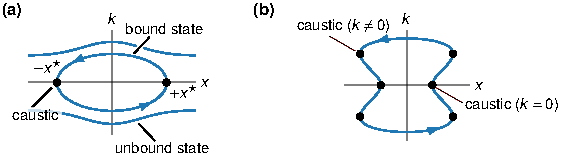
\includegraphics{localization/caustic.pdf}
  \end{center}
  \caption{%
    (a) In phase space, bound states are represented by rays in the form of closed orbits, which is analogous to that of a bound particle oscillating between two classical turning points ($\pm x^{\star}$ in the cartoon).
    Other trajectories represent unbound states.
    (b) A bound state represented by a ``peanut''-shaped orbit has six caustics.%
  }
  \label{fig:caustic}
\end{figure}

\section{Weyl symbols}

The Weyl symbol of an operator $\widehat{A}(x, \hat{k})$ is defined by
%
\begin{equation}
  A(x, k) = \int \dd{s}\, e^{-iks/\epsilon} \Bra{x + \tfrac{1}{2}s}\widehat{A}\Ket{x - \tfrac{1}{2}s}.
  \label{app:eq:weyl_def}
\end{equation}
%
A consequence of the above definition is that if operator $\widehat{A}$ is Hermitian with $\widehat{A}^{\dagger} = \widehat{A}$, then, taking the complex conjugate of Eq.~\eqref{app:eq:weyl_def}, we find
%
\begin{equation}
  A^{*}(x, k) = \int \dd{s}\, e^{+iks/\epsilon} \Bra{x + \tfrac{1}{2}s}\widehat{A}\Ket{x - \tfrac{1}{2}s}^{*}
  = \int \dd{s}\, e^{+iks/\epsilon} \Bra{x - \tfrac{1}{2}s}\widehat{A}\Ket{x + \tfrac{1}{2}s} = A(x, k),
  \label{eq:weylsym}
\end{equation}
%
showing that the symbol $A(x, k)$ is a real function of $x$ and $k$.
